% !TeX root = ../main.tex
\chapter{SLAM设计和实现}
一个SLAM系统的设计和实现是十分考究代码功底的。按流程一步步走确实能够写出一套能用的东西出来,但是再往上填东西就显得十分吃力。不仅如此,每张图片进入视觉历程计中都会产生上千个特征点每个特征点中一部分有对应的三维地图点,这些地图点又关联着每一个能够观测到它的图片,在BA的过程中还需要全局每一帧每一个地图点捆绑调整。点,图片,位姿,相机之间关系错综复杂,若是不能准确的理清之间的关系,很难编写出一套可用的SLAM框架。\par
除了逻辑上的困难,再一方面的困难就是编程语言上的困难。C++作为一门静态语言,在编写程序的时候要做好内存管理,线程安全等工作。将一个局部变量的地址传出去,释放或者访问已经被释放的内存空间等等这些问题对于初学者来说一不留神都可能遇到。而这些问题都是可以通过一定的编程规范来解决的,比如通过shared\_ptr或者unique\_ptr来保证内存的安全释放,绝不把回传局部变量的地址等等。好在C++11以及后续标准的不断提出,给人们编写大规模程序提供了更多安全上的保障。同时11标准还给C++添加了许多语法糖比如lambda表达式,auto,模板自动推导类型等等都让程序编写起来更加优雅易读。\par
\begin{figure}[H]
	\centering
	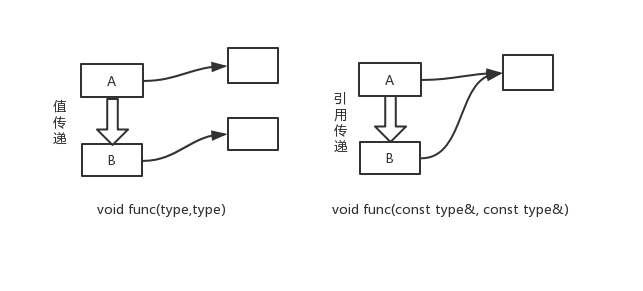
\includegraphics[height=7cm]{byvalueref}
	\caption{值传递和引用传递}
\end{figure}
再一方面就是效率上的问题,C++中函数的传入需要形参,这会使传入的量执行一次拷贝构造函数,同样的,在函数返回的时候要将返回值先执行一次拷贝构造函数,再把旧返回值析构掉。对于系统内置变量,这样的操作影响不大。但是对于用户自定义的类,特别是包含大量数据(比如图片)的成员变量来说,执行拷贝的代价是不可忍受的。因此我们可以采用const \&的方式来进行引用传递。或者可以让类不保存大型数据的实体,只保存地址以节省空间。在执行拷贝构造函数的时候只付出了拷贝地址的代价而不必拷贝实体。这些都能使程序的运行更加流畅。\par
SLAM是个增量式系统,图片会源源不断的读进程序中,如何保证程序不因为读入太多图片而导致内存爆炸,还需要及时从内存中释放掉一部分图片,考虑在相机静止不动的时候,由于一直有图片输入,系统就会不断地进行计算。我们肯定不希望整个模型变得越来越大,因此我们提出了关键帧的概念。对于非关键帧来说,它们的加入只是提供地图点然后就可以释放掉地图,而关键帧则需要留给后端做仔细的优化。\par
总之在实现一个SLAM系统的过程中,需要考虑的零零碎碎的东西非常之多,鉴于毕业设计时间仓促,并没有亲手实现出一整套SLAM系统。但是借助于航空学院赵勇博士的DIYSLAM\cite{zhao2019gslam}优秀的模块化设计,我得以实践SLAM中的很多模块。\par
下面就简单介绍一下SLAM的模块以及设计细节
\section{特征点匹配}
我们在前面介绍了很多特征点,现在我们就来看一下提取特征点的效率究竟如何:
\begin{table}[htbp]
	\centering
	\caption{特征点提取时间比较}
	\begin{tabular}{cccc}
		\toprule
		& 总耗时(ms) & 特征点数  & 单个特征点提取时间(ms) \\ \hline
		FAST   & 46.16   & 70829 & 0.0006        \\ \hline
		SIFT   & 3599.76 & 23458 & 0.1534        \\ \hline
		SURF   & 2761.82 & 43029 & 0.0641        \\ \hline
		ORB    & 114.77  & 500   & 0.2295        \\ \hline
		HARRIS & 439.42  & 1000  & 0.4394      	\\ \bottomrule
	\end{tabular}
\end{table}\par

\begin{table}[]
	\centering
	\caption{描述子计算时间比较}
	\begin{tabular}{cccc}
		\toprule
		& 总耗时(ms) & 特征点数 & 单个特征点描述子计算时间(ms) \\ \hline
		SIFT  & 958.15  & 500  & 1.9163           \\ \hline
		SURF  & 227.97  & 500  & 0.4559           \\ \hline
		ORB   & 144.90  & 500  & 0.2898           \\ \hline
		BRIEF & 26.46   & 500  & 0.0529          \\ \bottomrule
	\end{tabular}
\end{table}




